% This is samplepaper.tex, a sample chapter demonstrating the
% LLNCS macro package for Springer Computer Science proceedings;
% Version 2.21 of 2022/01/12
%
\documentclass[runningheads]{llncs}
%
\usepackage[T1]{fontenc}
% T1 fonts will be used to generate the final print and online PDFs,
% so please use T1 fonts in your manuscript whenever possible.
% Other font encondings may result in incorrect characters.
%
\usepackage{graphicx}
% Used for displaying a sample figure. If possible, figure files should
% be included in EPS format.
%
% If you use the hyperref package, please uncomment the following two lines
% to display URLs in blue roman font according to Springer's eBook style:
%\usepackage{color}
%\renewcommand\UrlFont{\color{blue}\rmfamily}
%\urlstyle{rm}
%
\usepackage{amsmath}    % Essential for advanced math formatting
\usepackage{amssymb}    % Provides additional mathematical symbols
\usepackage{amsfonts}   % Includes mathematical fonts (e.g., blackboard bold)
\usepackage{subcaption}
\usepackage[autolanguage]{numprint}
\usepackage{float}
\usepackage{booktabs}
\usepackage[colorlinks=true,        % Enables colored links
            linkcolor=blue,         % Color for internal links (e.g., table of contents)
            citecolor=blue,         % Color for citation links
            urlcolor=blue,          % Color for URLs
            breaklinks=true,        % Allows links to break over lines
            bookmarks=true,
            bookmarksdepth=3]{hyperref}

% Optionally, load the bookmark package for finer control over PDF bookmarks:
            \usepackage{bookmark}
            \usepackage{bbding}
            \usepackage{adjustbox}

% Manage acronyms
\usepackage[nolist]{acronym}

% ==================== prompt ====================

% You are computer science PhD professional. Your task is to assist me
% to improve the writing of scientific articles. This may involve
% summarize and re-phrase. The article is written in Latex so mastery
% in  the use of Latex is expected.

% You are computer science PhD professional. Your task is to assist me
% to improve the writing of scientific articles. This may involve
% rewriting or rephrase of provided text. The article is written in
% Latex. consequently, Latex syntax must be used. Also, if acronyms
% are found, consider  that they were previously defined. Also you may
% solve any question I have regarding machine learning or deep learning


% ==================== ICAI ID ====================
% PaperID: ICA9637
% ==================== ICAI ID  ====================
\begin{document}
%
% Setting acronyms in paper
\begin{acronym}
  \acro{EQA}[EQA]{Extractive Question Answering}
  \acro{NLP}[NLP]{Natural Language Processing}
  \acro{GAI}[GAI]{Generative Artificial Intelligence}
  \acro{QA}[QA]{Question Answering}
  \acro{AI}[AI]{Artificial Intelligence}
  \acro{LLMs}[LLMs]{Large Language Models}
  \acro{DL}[DL]{Deep Learning}
  \acro{LNLP}[LNLP]{Legal NLP}
  \acro{LQA}[LQA]{Legal Question Answering}
  \acro{RNNs}[RNNs]{Recurrent Neural Networks}
  \acro{LSTM}[LSTM]{Long Short-Term Memory}
  \acro{CNN}[CNN]{Convolutional Neural Networks}
  \acro{TF-IDF}[TF-IDF]{Term Frequency-Inverse Document Frequency}
  \acro{SQuAD}[SQuAD]{Stanford Question Answering Dataset}
  \acro{NER}[NER]{Named Entity Recognition}
  \acro{LDS}[LDS]{Legal Document Summarization}
  \acro{SVM}[SVM]{Support Vector Machine}
  \acro{GQA}[GQA]{Generative Question Answering}
  \acro{ZSL}[ZSL]{Zero-Shot Learning}
\end{acronym}
\title{Leveraging Transformer Models for Extractive Question Answering in Criminal Report Analysis}
%
\titlerunning{Leveraging Transformer Models for Extractive QA in Criminal Reports}
% If the paper title is too long for the running head, you can set
% an abbreviated paper title here
%
\author{Lenin G. Falconi\inst{1}\orcidID{0000-0003-4402-6643} \and\\
Lorena Isabel Barona López\inst{1}\orcidID{0000-0002-5184-3759}\and\\
Myriam Hernandez-Alvarez\inst{1}\orcidID{0000-0003-4718-0400}}
%
\authorrunning{L. Falconi et al.}
% First names are abbreviated in the running head.
% If there are more than two authors, 'et al.' is used.
%
% \institute{Princeton University, Princeton NJ 08544, USA \and
% Springer Heidelberg, Tiergartenstr. 17, 69121 Heidelberg, Germany
% \email{lncs@springer.com}\\
% \url{http://www.springer.com/gp/computer-science/lncs} \and
% ABC Institute, Rupert-Karls-University Heidelberg, Heidelberg, Germany\\
% \email{\{abc,lncs\}@uni-heidelberg.de}}

\institute{Escuela Politécnica Nacional, Quito 170525, Ecuador\\
\url{https://www.epn.edu.ec} \\
\email{\{lenin.falconi\Envelope, lorena.barona, myriam.hernandez\}@epn.edu.ec}}
%
\maketitle              % typeset the header of the contribution
% abstract 150 - 250 words

\begin{abstract}


  Transformer-based models have greatly advanced extractive question
  answering (EQA) in NLP, but their application to legal document
  analysis remains underexplored. This paper introduces a
  domain-adapted BERT model for EQA on Spanish-language robbery case
  reports from Ecuador’s Prosecutor's Office (\textit{Fiscalía General
    del Estado}). We used generative artificial intelligence to
  synthesize a SQuAD-format dataset tailored to robbery cases. The
  pre-trained BERT model was first evaluated in a zero-shot setting on
  this dataset, then further fine-tuned for the specific domain. The
  fine-tuned model outperformed the base version, achieving a final
  F1-score of 82.88. Our results demonstrate the effectiveness of
  transformer-based models, both in zero-shot and fine-tuned settings,
  for EQA tasks in legal language processing. These advancements
  highlight the potential to enhance information retrieval and
  optimize workloads in judicial systems, ultimately improving service
  delivery to communities.
  
\keywords{Legal Natural Language Processing \and NLP \and Natural
    Language Processing \and transformers \and LNLP \and law.}
\end{abstract}
%
%

\section{Introduction}
\label{sec:introduction}

Transformer-based models have emerged as powerful tools in \ac{NLP},
enabling more accurate and efficient extraction of relevant
information from complex texts such as criminal reports. These models
utilize self-attention mechanisms to weigh the importance of different
words in a sentence, allowing for better context understanding and
improved performance in tasks like \ac{QA}. By fine-tuning
these models on domain-specific datasets, researchers can enhance
their ability to discern pertinent details and provide precise answers
to inquiries related to criminal incidents.

The implementation of \ac{EQA} systems in legal contexts not only
enhances the efficiency of information retrieval but also addresses
challenges related to data variability and complexity inherent in
criminal reports. As these models are fine-tuned on diverse datasets,
they can improve their generalizability across different types of
legal documents, ensuring that critical details are accurately
captured regardless of nuances in language or
structure~\cite{jha2022extractive}. Moreover, recent advancements in
model architectures, such as the integration of dynamic masking
techniques, have shown promise in further refining performance by
enabling models to better adapt to varying levels of difficulty in
questions posed about complex
narratives~\cite{Pearce_Zhan_Komanduri_Zhan_2021}. This evolution
highlights the potential for transformer-based models to facilitate
more informed decision-making processes within the justice system,
ultimately contributing to enhanced outcomes for legal practitioners
and stakeholders alike.

The Prosecutor’s Office of Ecuador is responsible for handling a wide
range of cases, including criminal investigations and public safety
matters. Among these, robbery poses a significant challenge, with
\numprint{67705} reported incidents in
2024\footnote{\hyperref{https://www.fiscalia.gob.ec/analitica-cifras-de-robo/}{FGE's
    Theft Statistics}{FGE's Theft Statistics}{Statistics reported by
    FGE with data cut-off date June 13, 2025}} (equivalent to 376
robberies per \numprint{100000} inhabitants). The comprehensive
analysis of these crime reports serves multiple critical functions:
(1) it enables more effective investigations by revealing criminal
patterns, (2) supports victims' insurance claims for stolen property,
and (3) provides essential data for public safety planning. \Ac{AI} is
particularly valuable in this context, as automated systems can can
enhance the efficiency of processing case information, alleviate
backlogs, and ultimately improve service delivery to citizens.

Our previous research investigated robbery classification using
state-of-the-art neural architectures, with a focus on fine-tuned
language models. Extending this work, the current study investigates
the application of \ac{EQA} systems for processing criminal
reports. The proposed methodology demonstrates significant potential
to assist legal authorities by: (1) extracting actionable insights for
criminal investigations, and (2) enabling comprehensive crime
statistics analysis. To our knowledge, this represents the first
application of transformer-based models utilizing a specially curated
Spanish-language \ac{SQuAD} dataset derived from Ecuadorian legal
documents.

This paper is organized as follows:
Section~\ref{sec:literature-review} surveys existing applications of
\ac{AI} in legal domains, with a focus on question answering (\ac{QA})
tasks and discusses important concepts such as \ac{GAI} and
\ac{ZSL}. Section~\ref{sec:methodology} describes our methodology,
including dataset construction and model
training. Section~\ref{sec:results} presents the comparative results
of the \ac{ZSL} model and the fine-tuned model. Finally,
Section~\ref{sec:conclusions} summarizes our main findings and
outlines opportunities for future work.

% \newpage

\section{Literature Review}
\label{sec:literature-review}

\Ac{LLMs} represent a category of \ac{DL} models that
integrate transformer architectures with large-scale pre-training on
extensive text corpora. Trained in a self-supervised fashion, these
models capture detailed linguistic patterns and can subsequently be
fine-tuned to address domain-specific challenges in~\ac{LNLP}. For
instance, one influential model is described in~\cite{devlin2018bert},
and another is presented in~\cite{radford2018gpt}, where OpenAI
reported that the model achieved performance at the 90th percentile on
the Uniform Bar Exam, a standardized examination used to evaluate the
competency of prospective attorneys. However, subsequent analysis
by~\cite{Martinez2024} indicates that GPT-4's actual performance
ranges from the 48th to the 62nd percentile. These authors critique
the imprecision and lack of transparency in OpenAI's report, arguing
that such shortcomings may hinder the development of safe \ac{AI} and
lead to misconceptions regarding the model's true capabilities in
handling complex legal tasks.

\Ac{LQA} is a complex task that entails addressing queries related to
legal issues, necessitating not only the analysis of extensive legal
corpora but also their nuanced interpretation~\cite{Ariai2024}. A wide
range of models and algorithms have been explored for \ac{QA} in
\ac{NLP}, such as \textit{\ac{RNNs}}, \textit{\ac{LSTM}}, and
\textit{\ac{CNN}}. Additionally, information retrieval approaches,
including \textit{\ac{TF-IDF}}, are frequently utilized. Both
extractive and generative methodologies have demonstrated
effectiveness in addressing \ac{NLP}-based \ac{QA}
tasks~\cite{Luo2022NLP}.

It is important to clarify the primary distinction between these two
approaches. \Ac{EQA} identifies and retrieves a span of text
directly from the given context: Given a tuple composed of the
question $q$ and the context $c$, the model predicts the
start and end positions of the answer. In contrast, \ac{GQA}
synthesizes responses using encoder-decoder architectures, generating
answers in an autoregressive manner~\cite{Luo2022NLP}. According to a
systematic evaluation of \ac{QA} models by~\cite{Luo2022NLP}, generative
readers generally outperform extractive readers with longer contexts,
providing more fluent and comprehensive answers, whereas extractive
readers are more effective when the context is limited and exhibit
better out-of-domain generalization.


\subsection{Large Language Models and Generative AI}
\label{sec:large-lang-models}

\Ac{GAI} refers to a class of \ac{AI} models that learn the underlying
data distribution $p_{data}(\mathbf{x})$ to generate novel samples
(e.g., text, images, or audio) through an estimated model distribution
$p_{model}(\mathbf{x})$~\cite{foster2022generative}. Modern \ac{AI}
models are considered Foundational Models, which represent a class of
general-purpose models capable of handling diverse data modalities and
supporting multiple \ac{AI} tasks~\cite{Grattafiori2024}. Notable
examples include the Llama 3 family of models, which are foundational
language models featuring multilingual capabilities, programming
proficiency, reasoning skills, and tool
integration~\cite{Grattafiori2024}. Equation \eqref{eq:gai-def}
represents the goal of \ac{GAI}, which is to to learn a model
distribution $p_{model}(\mathbf{x})$ that approximates the true data
distribution $p_{data}(\mathbf{x})$, where $\mathbf{x}$ represents
observations from the data domain.


\begin{equation}
  \label{eq:gai-def}
  p_{model}(\mathbf{x}) \approx p_{data}(\mathbf{x})
\end{equation}


\Ac{LLMs} are a specialized subset of foundational \ac{AI} and
\ac{GAI} models, with a primary focus on text-based tasks. These
models leverage transformer
architectures~\cite{Grattafiori2024,Minaee2025} and undergo extensive
pre-training on textual corpora. Notably, \ac{LLMs} exhibit
exceptional capabilities in natural language understanding and complex
problem-solving (i.e., General Purpose Task Solver)~\cite{Zhao2023},
rendering them particularly effective for sophisticated linguistic
tasks. The basic working of an \ac{LLMs} can be thought of as a
next-word prediction problem, where given a sequence of tokens
$\mathbf{x}_{1:t} = (x_1, \ldots, x_t)$, an LLM defines a conditional
probability distribution over the vocabulary $\mathcal{V}$:

\begin{equation}
  \label{eq:llm-def}
P(x_{t+1} | \mathbf{x}_{1:t}; \theta) = \text{softmax}(\mathbf{W} \cdot \mathbf{h}_t + \mathbf{b})
\end{equation}

$\theta$ denotes the model parameters, and $\mathbf{h}_t$ is obtained
by several layers of transformer blocks that process an embedded
representation of the tokenized text:

\begin{equation}
\mathbf{h}_t = \text{Transformer}(\mathbf{x}_{1:t}; \theta)
\end{equation}

\subsection{Zero-Shot Learning}
\label{sec:zero-shot-learning}

Traditional supervised learning in \ac{DL} requires large labeled
datasets, which can be difficult and expensive to
obtain~\cite{Rampur2018}. For instance, the \ac{SQuAD} 2.0 benchmark
dataset for \ac{EQA} contains approximately \numprint{150000} samples
(\numprint{100000} answerable and \numprint{50000}
unanswerable)~\cite{rajpurkar2018}. In this context, \ac{ZSL}
establishes a new paradigm in machine learning, where models trained
on a subset of classes are expected to recognize new classes not seen
during training~\cite{Ramesh2025}. Consequently, \ac{ZSL} addresses
the challenge posed by unlabeled data~\cite{Rampur2018}. Moreover,
pre-trained language models (e.g., BERT) that are trained on
large-scale corpora achieve strong performance in \ac{ZSL} by encoding
linguistic patterns.

Transfer learning aims to utilize knowledge from a source domain to
improve performance in a target domain with limited labeled data,
typically through fine-tuning pre-trained language
models~\cite{Ramesh2025}. However, this fine-tuning process can lead
to catastrophic forgetting, where the model loses its original
capabilities while adapting to new tasks. In contrast, \ac{ZSL} does
not require explicit labeling~\cite{YuchenGuo2018}, thereby preserving the
model's original knowledge while enabling generalization to unseen
classes.

In this research, we explore \ac{ZSL} on the Legal \ac{EQA}
domain using a new set of samples from our dataset. Traditional
applications in \ac{NLP} include text classification, sentiment
analysis, and \ac{NER}~\cite{Rampur2018}. Our approach relies on the
use of pre-trained language models such as BERT, which are powerful
tools for \ac{ZSL}. However, other \ac{ZSL} techniques are: semantic
embedding, attribute-based approaches, and
generative~\cite{Ramesh2025,Rampur2018}


\subsection{Related Works}
\label{sec:related-works}

There is significant interest within both the scientific community and
legal institutions in studying the applications of \ac{AI} in this
expansive field. The current state of the art in \ac{NLP} with DL
primarily focuses on the use of transformer-based architectures, which
have demonstrated superior performance across various \ac{NLP}
tasks. However, improvements over this architecture are discussed
in~\cite{Shao_Guo_Chen_Zepeng_2019}, where a Bidirectional Long
Short-Term Memory (BiLSTM) layer is integrated with the transformer to
capture both global and sequential features. Although, their work is
limited to natural language domain, the authors show that hybrid
architectures with varied pooling strategies may improve
state-of-the-art performance in \ac{QA}.

In~\cite{Vold_Conrad_2021}, the deployment of a RoBERTa Base \ac{QA}
classification model specifically for legal questions is discussed.
It compares the performance of this transformer model against a
traditional linear \ac{SVM} in the legal domain, using the PRIVACYQA
dataset. The results indicate that RoBERTa significantly outperforms
the \ac{SVM}, achieving a 31\% improvement in F1-score and a 41\%
improvement in Mean Reciprocal Rank, demonstrating the effectiveness
of transformers in enhancing answer retrieval for legal inquiries.

For information retrieval,~\cite{Kim_Rabelo_Babiker_Rahman_Goebel_2024} discuss the use of
transformer-based approaches for legal information retrieval and
entailment, specifically in the context of the COLIEE competition. For
case law retrieval, a sentence-transformer model was employed
to create numeric representations of case paragraphs, facilitating
similarity assessments. As for the  entailment task, a fine-tuned DeBERTa
large language model was utilized, achieving third place among eight
teams. These methods demonstrate the effectiveness of transformers in
addressing \ac{LQA} challenges.

Another area of interest is predicting legal
judgments. In~\cite{Ghosh_Kumar_2024} six transformer-based models
(BERT, XLNet, RoBERTa, DeBERTa, ELECTRA, and BigBird) are evaluated in
predicting legal judgments using the ILDC dataset. It highlights the
potential of these models in automating legal decision-making, with
newer models achieving up to 80\% accuracy compared to 76\% for older
models. This comparative analysis underscores the advancements in
\ac{NLP} technology and its applicability in the legal domain,
suggesting a promising future for \ac{QA} in law through transformer
models.

Finally, in \cite{Peric_Mijic_Stammbach_Ash_2020} the use of
transformers to generate legal text is addressed, indicating their
potential to assist in legal practice. The findings suggest that these
models can effectively generate judicial opinions and help
differentiate between human and machine-generated legal texts, which
could be beneficial for tasks like drafting contracts and briefs,
although direct application to \ac{QA} is not discussed.

The reviewed studies indicate that transformer-based architectures
have become the dominant approach in \ac{LNLP}, either through
fine-tuning or architectural modifications. Applications include
information retrieval, judgment prediction, and legal text
generation. These trends highlight the relevance of the present work
in addressing the \ac{LQA}.
\newpage
\section{Methodology}
\label{sec:methodology}
In this paper, we present a BERT-based model fine-tuned for \ac{EQA}
on Spanish-language criminal reports. We started from a Spanish BERT
architecture already pre-trained and optimized for \ac{QA} tasks, then
fine-tuned it to extract information from robbery crime narratives. Our
methodology consists of three phases: (1) dataset generation, (2)
\ac{ZSL} pre-trained model performance, and (3) model fine-tuning.


\subsection{Phase 1: Robbery Crime QA Dataset Generation}
\label{sec:robb-crime-quest}

% Meta-Llama-3-8B-Instruct
\subsubsection{Data Collection and Preprocessing}
\label{sec:data-collection}
We constructed our dataset using a set of unlabeled robbery crime
reports. The text preprocessing pipeline involved removing
non-alphanumeric characters and converting all text to
lowercase. Statistical analysis of the collected reports revealed an
average length (mean) of 112 words, and an upper bound of 150
words. Consequently, we included reports $x_i$ satisfying
$82 \leq \Gamma(x_i) \leq 150$, where
$\Gamma: x_i \rightarrow \mathbb{N}$ denotes the word count function
for report $x_i$. This filtering criterion effectively removed
statistical outliers while maintaining the core
distribution. Figure~\ref{fig:dataset-visualizations} illustrates the
word count distribution across the original dataset of
\numprint{174594} samples, presented through both histogram and box
plot visualizations. Finally, we transformed this dataset into a
\ac{QA} format compatible with \ac{SQuAD} using \ac{GAI}.


% \begin{figure}[]
%   % \centering                    %
%   \begin{subfigure}[b]{\linewidth}
%     \includegraphics[width=.8\linewidth]{./images/histogramOriginalDatasetPadded.png}
%     \caption{Original Dataset Histogram}
%     \label{fig:histogram-original-dataset}
%   \end{subfigure}
  
%   \vspace{0.1cm} % Add some vertical space between the subfigures
  
%   \begin{subfigure}[b]{\linewidth}
%     \includegraphics[width=.8\linewidth]{./images/boxPlotOriginalDatasetPadded.png}
%     \caption{Box plot of Words Length in Original Dataset}
%     \label{fig:boxplot-original}
%   \end{subfigure}
  
%   \caption{Distribution of word counts in collected data visualized through (a) a histogram  and (b)  a box plot}
%   \label{fig:dataset-visualizations}
% \end{figure}

\begin{figure}[ht]
  \centering
  \begin{subfigure}[t]{0.48\linewidth}
    \includegraphics[width=\linewidth]{./images/histogramOriginalDatasetPadded.png}
    \caption{Original Dataset Histogram}
    \label{fig:histogram-original-dataset}
  \end{subfigure}
  \hfill
  \begin{subfigure}[t]{0.48\linewidth}
    \includegraphics[width=\linewidth]{./images/boxPlotOriginalDatasetPadded.png}
    \caption{Box Plot of word counts}
    \label{fig:boxplot-original}
  \end{subfigure}
  \caption{Distribution of word counts in collected data presented as
    (a) histogram and (b) boxplot. The histogram shows a right-skewed
    distribution of crime reports. The interquartile range spans from
    82 to 150 words, with a median of 112 words.}
  \label{fig:dataset-visualizations}
\end{figure}

% \begin{figure}[ht]
%   \centering
%   \begin{subfigure}[b]{0.48\linewidth}
%     \adjustbox{valign=t}{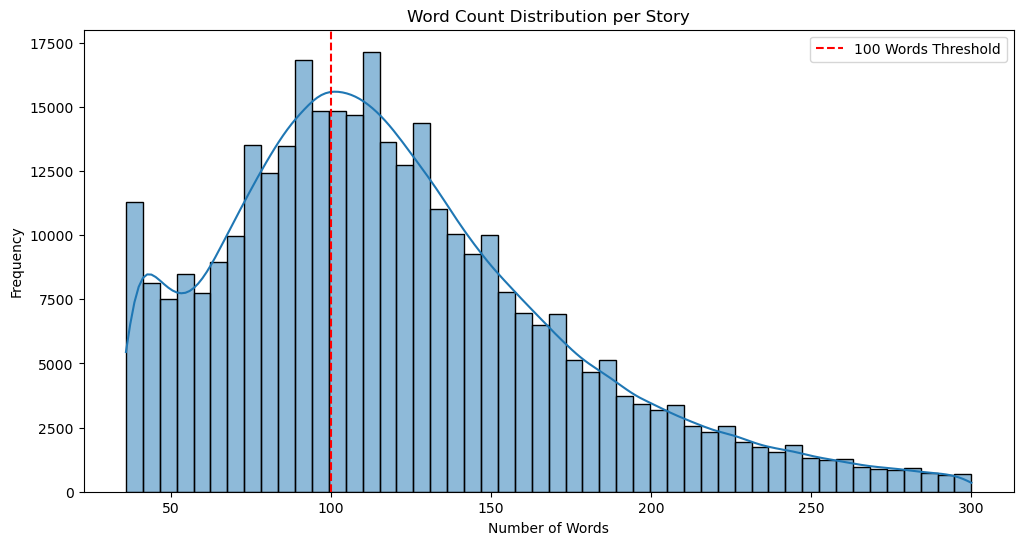
\includegraphics[width=\linewidth,height=6cm,keepaspectratio]{./images/histogramOriginalDataset.png}}
%     \caption{Original Dataset Histogram}
%     \label{fig:histogram-original-dataset}
%   \end{subfigure}
%   \hfill
%   \begin{subfigure}[b]{0.48\linewidth}
%     \adjustbox{valign=t}{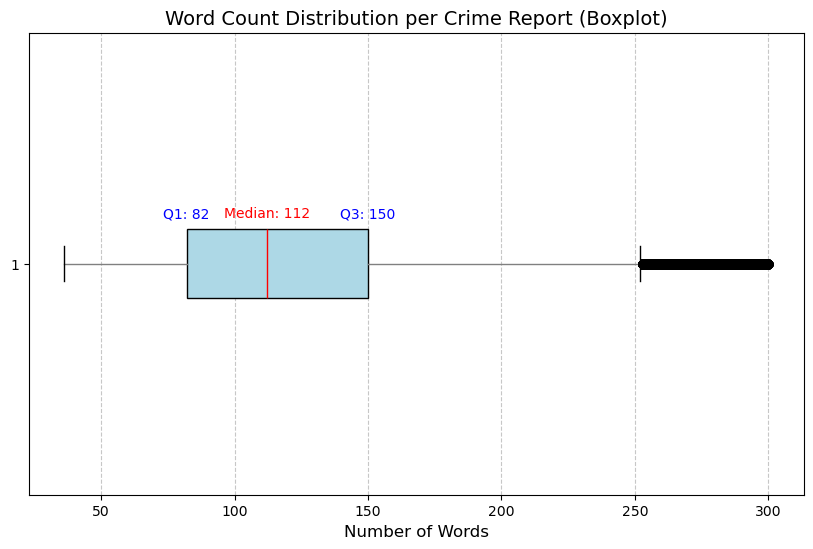
\includegraphics[width=\linewidth,height=6cm,keepaspectratio]{./images/boxPlotOriginalDataset.png}}
%     \caption{Box Plot}
%     \label{fig:boxplot-original}
%   \end{subfigure}
%   \caption{Distribution of word counts in collected data}
%   \label{fig:dataset-visualizations}
% \end{figure}


% Meta-Llama-3-8B-Instruct
\subsubsection{Generative AI Prompt Engineering}
\label{sec:prompt-engin-gai}


For this research, we used
Meta-\textsc{Llama}-3-8B-Instruct~\cite{llama3modelcard}, an
instruction-tuned variant of Meta’s \textsc{Llama}~3 8B parameter
language model, optimized for conversational and task-oriented
interactions with multilingual capabilities. Built on a decoder-only
\textsc{Transformer} architecture, it leverages supervised fine-tuning
(\textsc{SFT}) and reinforcement learning from human feedback
(\textsc{RLHF}) to align responses with user intent. The model is
pre-trained on a diverse corpus of publicly available text data, with
enhancements in reasoning, coding, and safety mitigation compared to
its predecessors.

Prompt engineering is the process of crafting a suitable prompt to
drive the \ac{LLMs} to solve a complex task, using natural language
text~\cite{Zhao2023}. In this work, the LLM functions as an expert
data science assistant with the goal of constructing a dataset in the
\ac{SQuAD} format in Spanish. For this purpose, the prompt receives
the content of the crime report as the \texttt{context} and each of
the questions from Table \ref{tab:commonquestions} as the
\texttt{question}. The LLM was also instructed to retrieve a
\texttt{json} format output with the variables: \texttt{context},
\texttt{question}, \texttt{answer\_text}, \texttt{answer\_start},
\texttt{answer\_end}, and \texttt{impossible\_find\_answer}. The
latter was calculated by finding the \texttt{answer\_text} in the
context. In the case that no answer was possible to be retrieved,
either because there is no answer or because the LLM failed, the
variable \texttt{impossible\_find\_answer} was set to True.

\begin{table}[h]
  \centering
  \small
\caption{Proposed Questions for the Dataset}
\label{tab:commonquestions}
\begin{tabular}{|p{0.9\textwidth}|}
\hline
\textbf{Question} \\
\hline
What objects were stolen? \\
% \hline
On what date did the incident occur? \\
% \hline
At what time did the robbery happen? \\
% \hline
At what address or between which streets did the robbery/incident occur? \\
% \hline
What was the dollar value of the stolen or taken objects? \\
\hline
\end{tabular}
\end{table}

Hugging Face's Inference API processed samples at a speed of 6.4
samples per minute. A total of \numprint{1544} samples were obtained after four
hours. Our evaluation revealed two key limitations of the LLM: (1)
incomplete retrieval of answers for certain queries, and (2) sporadic
generation of irrelevant content. These results suggest that manual
verification of the generated dataset can aid in improving
quality. However, the engineered prompt allowed for the identification
of problems in generated samples.
\subsubsection{Dataset Quality}
\label{sec:dataset-quality}
After collecting the initial \numprint{1544} samples, which generated
\numprint{7705} question-answer pairs at five questions per context,
we conducted quality assessment using the
\texttt{impossible\_find\_answer} flag. This process identified
approximately \numprint{3000} invalid cases, leading us to retain only
samples where \texttt{impossible\_find\_answer} is
\texttt{False}. Through histogram and box plot analysis of answer
lengths, we established an upper limit of 17 words for valid
responses. The final curated dataset consisted of \numprint{4572}
samples, all containing at least one word and meeting our validity
criteria, suitable for model training and evaluation.


\subsubsection{Dataset Train and Test Split}
\label{sec:dataset-split}
The dataset was partitioned into training and testing sets, with 20\%
of the samples allocated for evaluation. The remaining 80\% were used
for training. This approach is a fundamental machine learning
technique that helps to evaluate the model's performance and
generalization capability. Table~\ref{tab:org63e879b} summarizes the
sample sizes for each subset. The split was performed randomly.

\begin{table}[htbp]
\caption{\label{tab:org63e879b}Dataset Train and Test Split}
\centering
\small
\begin{tabular}{lr}
  \hline
Partition & \# Samples\\[0pt]
\hline
Train & \numprint{3657}\\[0pt]
  Test & \numprint{915}\\[0pt]
  \hline
  Total & \numprint{4572}\\[0pt]
  \hline
\end{tabular}
\end{table}
% check from here

\subsection{Phase 2: Zero Shot Learning Pre-Trained Model Performance}
\label{sec:phase-2:-baseline}


We selected the
\texttt{mrm8488/bert-base-spanish-wwm-cased-finetuned-spa-squad2-es}
model as the baseline pre-trained model due to its specialization for
Spanish language processing in \ac{QA} tasks. This model represents a
distilled version of BETO (Spanish BERT)~\cite{CaneteCFP2020} that was
further fine-tuned on the SQuAD-es-v2.0 dataset. The architecture
follows the standard BERT-base~\cite{devlin2018bert} configuration,
featuring:
\begin{itemize}
    \item 12 Transformer blocks
    \item 768-dimensional hidden states
    \item 12 self-attention heads
    \item 384 tokens of sequence length
\end{itemize}

BETO was pretrained on an extensive Spanish corpus using Whole Word
Masking. In preliminary testing without additional fine-tuning, the
model achieved an F1-score of 81.70, demonstrating strong baseline
performance for Spanish \ac{QA} tasks.

\subsection{Phase 3: Model Fine-Tuning}
\label{sec:model-fine-tuning}
To fine-tune the pre-trained model, both the question and the answer
need to be tokenized. As a result of this process, the indices
indicating the start and end of the answer must be recalculated based
on the tokenized embedding. In the case of long text, truncation
should be applied only to the context, and a window of 128 tokens was
used to avoid losing the answer during truncation. However, in this
scenario, since most of the current samples have no more than 100
words in the context, this issue is unlikely to occur; nonetheless, it
has been addressed in the program.

In order to train the model, the parameters shown in Table
\ref{tab:org68816bf} were used. A small learning rate is recommended
for fine-tuning in order to reuse the pre-training from the original model and
adapt the new model to the target dataset. Our results prove that it
is possible to achieve a better performance on the target domain with
the fine-tuned model rather than using the pre-trained model. Although
the difference in performance is small, it could be related to the
fact that we were not able to use the whole dataset.

\begin{table}[htbp]
\caption{\label{tab:org68816bf}Training Parameters}
\centering
\small
\begin{tabular}{ll}
  \hline
Parameter & Value\\[0pt]
\hline
Strategy & epoch\\[0pt]
Learning rate & \(2 \times 10^{-5}\)\\[0pt]
Batch Size & 64\\[0pt]
Epochs & 10\\[0pt]
Weight Decay & 0.01\\[0pt]
FP16 & True\\[0pt]
  Metric for best model & F1 (eval)\\[0pt]
  \hline
\end{tabular}
\end{table}

\section{Results}
\label{sec:results}

In this section, we present the results of fine-tuning the model,
along with the performance of the pre-trained model on the test
set. This comparison was conducted to determine whether the fine-tuned
model demonstrates any improvement over \ac{ZSL}. Table
\ref{tab:comparative-results} shows the performance of each learning
approach used in this research.

Fine-tuning improves upon \ac{ZSL} in terms of F1 score and exact
match, with values of 82.88 and 81.70, respectively, indicating higher
accuracy. The exact match metric measures the percentage of
predictions that match any ground truth answer exactly. However, the
pre-trained model used in \ac{ZSL} shows lower evaluation loss and
higher steps per second, suggesting less error and greater
throughput. Thus, while fine-tuning yields better accuracy, the
\ac{ZSL} model is slightly less accurate but faster.

Our results suggest that increasing the number of samples for the
fine-tuning approach may improve model performance. It is also
important to note that the use of \ac{GAI} enabled the synthesis of a
training dataset through prompt engineering. According
to~\cite{Ramesh2025} and~\cite{Rampur2018}, this represents another
application of \ac{ZSL}.


\begin{table}[ht]
  \centering
  \caption{Comparison of Pre-trained and Fine-tuned Model Performance}
  \label{tab:comparative-results}
  \small
  \begin{tabular}{lrr}
\toprule
Metric & Zero Shot & Fine-tuning \\
\midrule
eval\_loss                   & 0.9102  & 1.0088    \\
eval\_model\_preparation\_time & 0.0077  & 0.0077    \\
eval\_exact                  & 53.5519 & 55.7377   \\
eval\_f1                     & 81.7041 & 82.8805   \\
eval\_total                  & 915.0000 & 915.0000 \\
eval\_HasAns\_exact          & 53.5519 & 55.7377   \\
eval\_HasAns\_f1             & 81.7041 & 82.8805   \\
eval\_HasAns\_total          & 915.0000 & 915.0000 \\
eval\_best\_exact            & 53.5519 & 55.7377   \\
eval\_best\_exact\_thresh    & 0.0000  & 0.0000    \\
eval\_best\_f1               & 81.7041 & 82.8805   \\
eval\_best\_f1\_thresh       & 0.0000  & 0.0000    \\
eval\_runtime                & 12.3982 & 12.8109   \\
eval\_samples\_per\_second   & 73.8010 & 71.4240   \\
eval\_steps\_per\_second     & 1.2100  & 1.1710    \\
epoch                       & --      & 10.0000   \\
\bottomrule
  \end{tabular}
\end{table}

\newpage
\section{Conclusions and Future Works}
\label{sec:conclusions}
In this study, we demonstrated the effectiveness of transformer-based
models for \ac{EQA} within the context of criminal report
analysis. Our fine-tuned model showed achieved an F1 score of 82.88,
improving upon the pre-trained model's zero-shot score of 81.70. This
indicates the potential for enhanced performance through
domain-specific fine-tuning. It also shows that \ac{ZSL} can achieve a
reasonable performance with a higher throughput.

The proposed methodology could be extended to other legal contexts in
other countries, provided a pre-trained \ac{QA} model in the target
language is available. According to our results, a zero-shot approach
achieves good performance. However, based on our experience,
fine-tuning the model increases performance. Additionally, using
\ac{GAI} to create a \ac{SQuAD} dataset can be adapted to the new
target.

The application of our model to robbery crime reports could facilitate
the extraction of crucial information, supporting legal practitioners
in their investigations and reporting. However, the study also
highlighted some limitations, including the model's occasional
inability to retrieve accurate answers and the need for manual
verification of results.

Future work will address current limitations by exploring advanced
techniques and incorporating manual dataset labeling by expert
peers. Additional computational resources will be necessary for larger
datasets. Integrating AI into the legal domain offers significant
potential for improved case management and resource allocation,
promoting a safer community. Further research should assess the impact
of AI in the legal field, particularly regarding data and
methodological biases. Exploring other NLP approaches, such as Legal
Legal \ac{NER} and \ac{LDS}, within the Ecuadorian context is also
recommended. Continued research and collaboration are encouraged to
refine these methods and maximize AI's benefits in supporting the
justice system.



\begin{credits}
  \subsubsection{\ackname}
  The authors would like to thank to the Faculty of Systems
  Engineering at Escuela Politécnica Nacional in Quito, Ecuador, for
  providing both academic guidance and financial support. We are
  equally indebted to the Fiscalía General del Estado for their
  cooperation in the development of this research.

\subsubsection{\discintname}
The authors have no competing interests to declare that are relevant
to the content of this article.
\end{credits}
%
% ---- Bibliography ----
%
% BibTeX users should specify bibliography style 'splncs04'.
% References will then be sorted and formatted in the correct style.
%
\bibliographystyle{splncs04}
\bibliography{bibliography}
% splncs04 was modified from line 461 to 567 to adjust to no more than
% 6 authors per reference
% 
\end{document}

%%% Local Variables:
%%% mode: LaTeX
%%% TeX-master: t
%%% End:
